\chapter*{Morphology-Density Appendix} \label{chap:morph_den_ap}

\section{Separation into Star-Forming \& Quiescent Sub-populations} \label{sec_c4:ap:cc_sel}

To separate the galaxies in our sample into star-forming and quiescent sub-populations, we follow \citet{Kawin16} and \citet{hsc_mass_size}. We begin by defining a generic region on the \textit{urz} color-color diagram for quiescent galaxies:-

\begin{equation}
    \begin{aligned}
        u-r & >A \times(r-z)+\mathrm{ZP} \\
        u-r & >(u-r)^{\prime} \\
        r-z & <1.15
\end{aligned}
\label{eq_c4:color-color}
\end{equation}

\noindent where A, ZP, and $(u-r)^{\prime}$ are variables that we derive using galaxies in each redshift slice with stellar masses above the overall stellar mass completeness limit. 

\begin{table}[htbp]
    \centering
    \caption{Best Fit Values For Eq. \ref{eq_c4:color-color}  \label{tab_c4:color-color}}
    \begin{tabular}{cccc}
    \hline
    \hline
     Redshift Slice & $(u-r)^{\prime}$ & A & ZP \\
     \hline
     \hline
     $0.3 \leq z < 0.4$ & 1.75 & 2.75 & 0.40 \\
     $0.4 \leq z < 0.5$ & 1.87 & 3.07 & 0.23 \\
     $0.5 \leq z < 0.6$ & 1.83 & 3.48 & -0.05 \\
     $0.6 \leq z < 0.7$ & 1.83 & 3.52 & -0.02 \\
     \hline
     \hline
    \end{tabular}
\end{table}

First, we measure $(u-r)^{\prime}$ as the local minima between the two peaks observed in the \uband-\rb{} color distribution (see the upper panels of Figure \ref{fig_c4:color_sep}). Thereafter, we derive the value of $A$ in Eq. \ref{eq_c4:color-color} by fitting the slope of the red sequence in the \textit{urz} diagram. Once the slope of the line has been fixed, we need to place it at an optimal location in the diagram. For this, we measure the \textit{urz} color distance of all galaxies from the line defined by the slope $A$ in Eq. \ref{eq_c4:color-color}. Finally, we set zero-point $ZP$ as the local minima between the two peaks in the measured \textit{urz} color distance distribution. 

\begin{figure*}[htb]
    \centering
    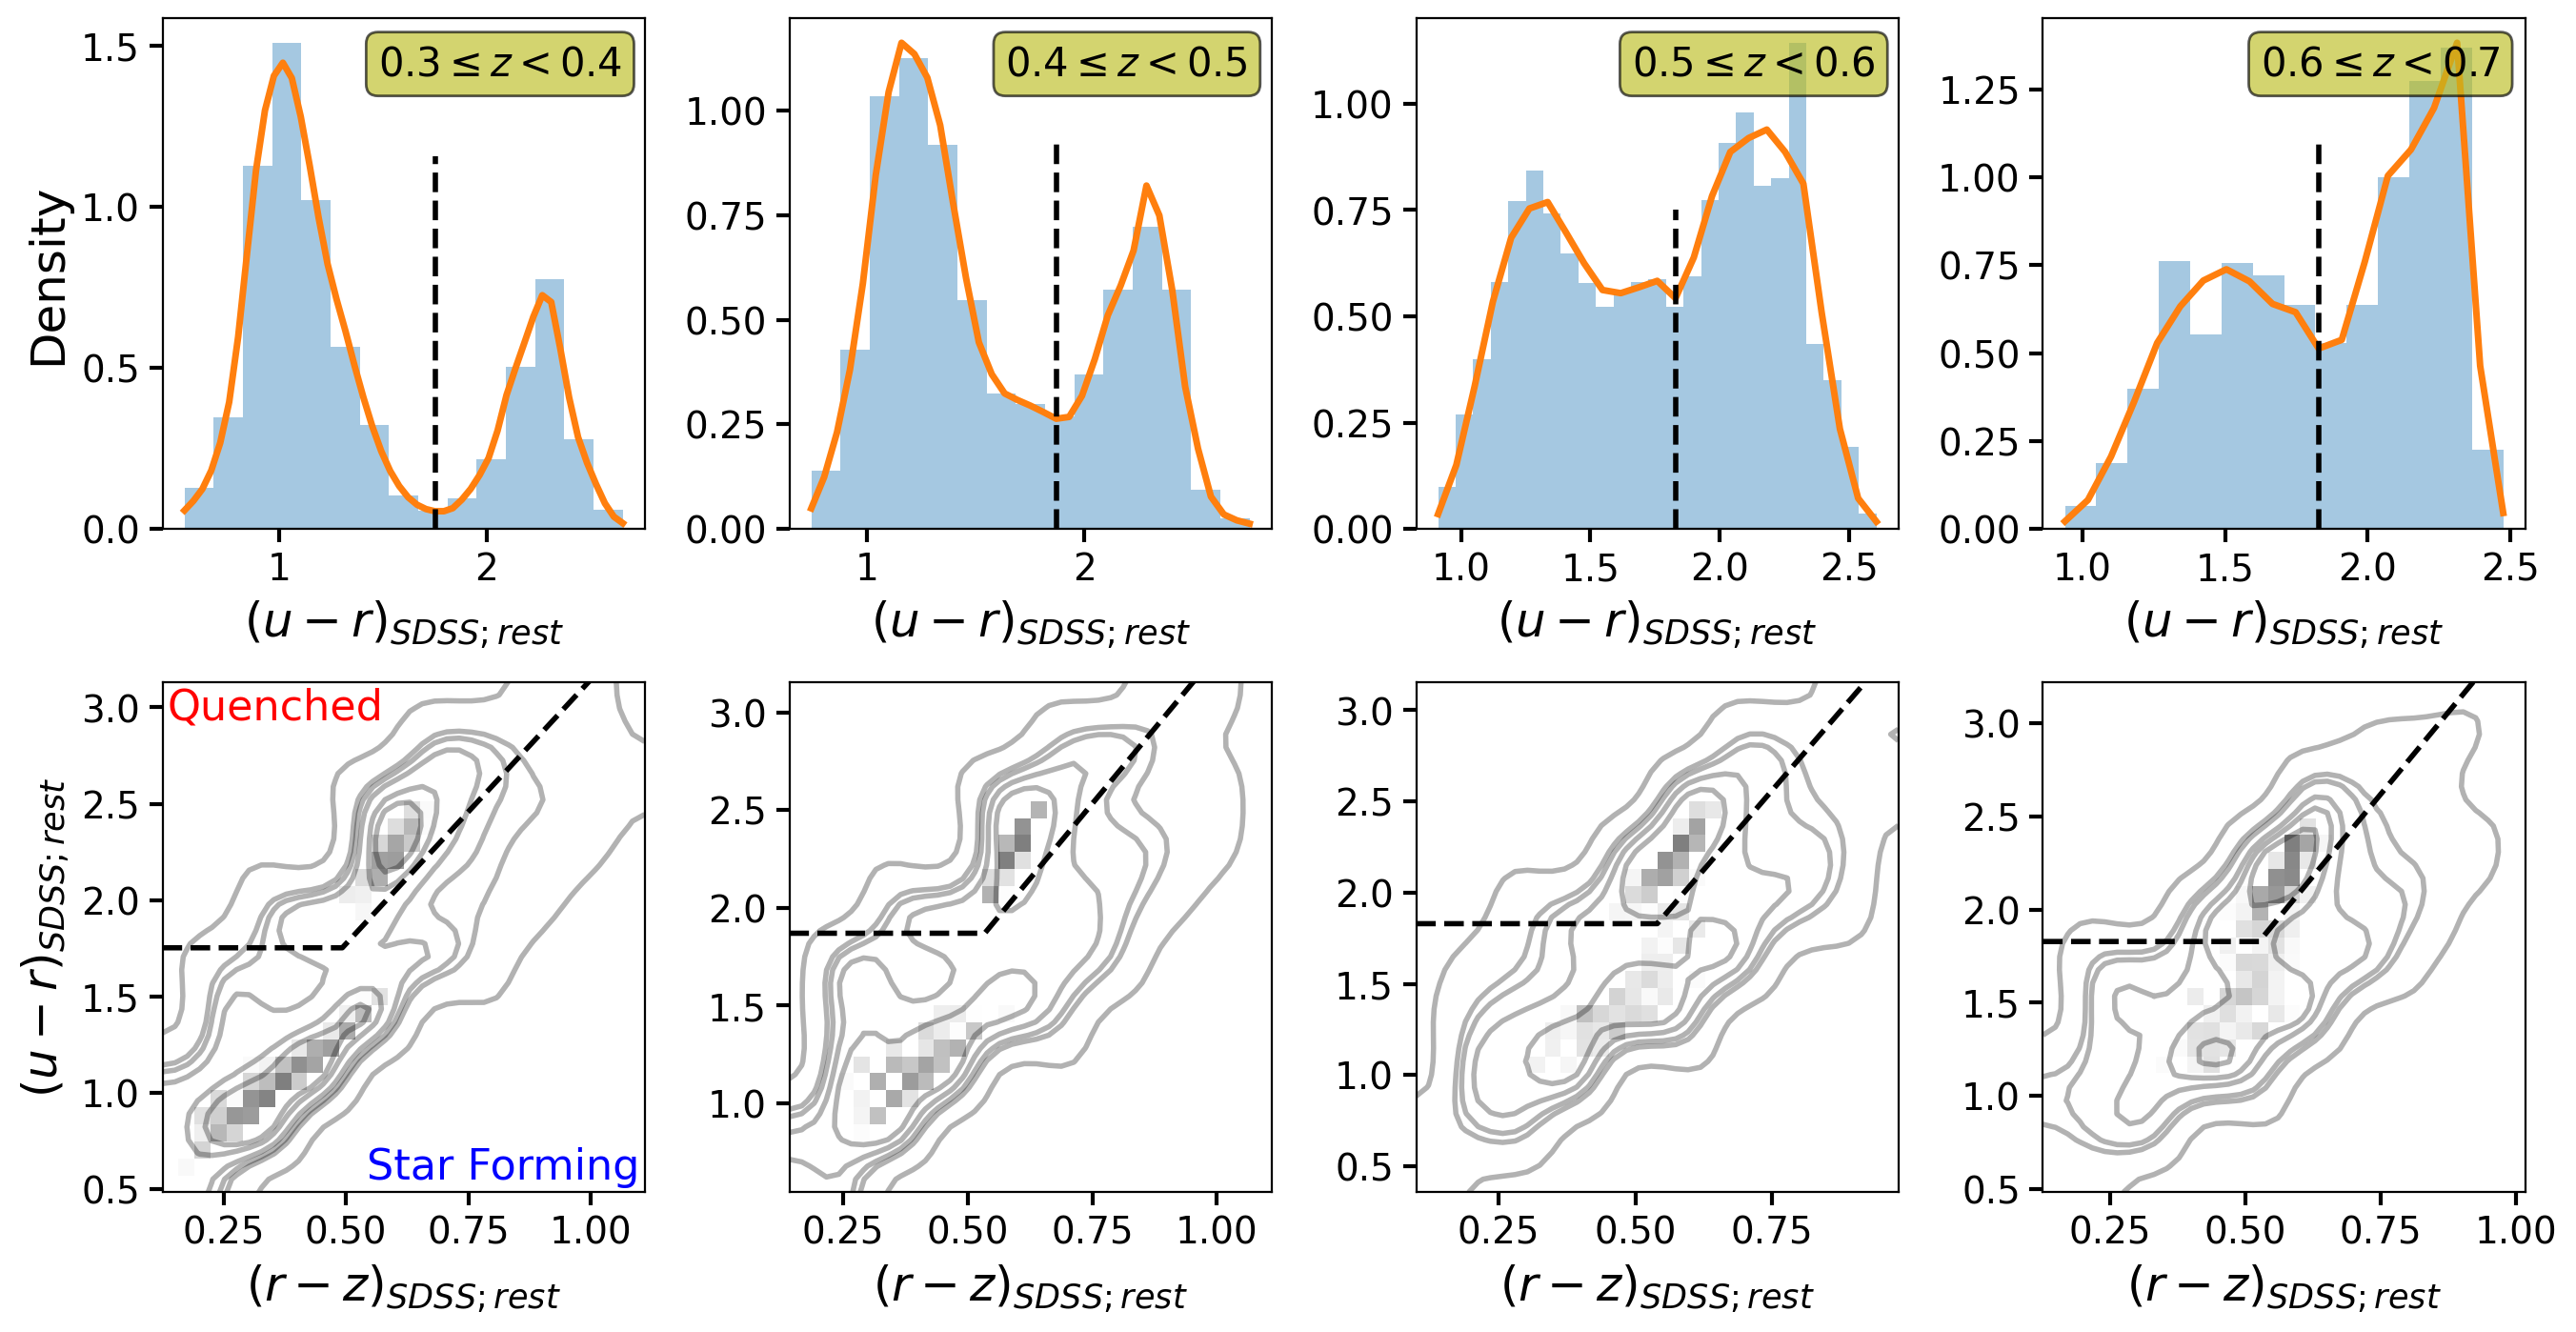
\includegraphics[width = \textwidth]{color_sep.png}
    \caption{ (\textit{Top Row}): The distribution of SDSS rest-frame \uband{}-\rb{} colors are shown for the four different redshift slices. The solid orange lines depict kernel density estimation (KDE) fits to ascertain the \uband{}-\rb{} probability density function. The dashed vertical line marks the local minima (obtained using the KDE estimate) between the two peaks of the \uband{}-\rb{} distribution. (\textit{Bottom Row}): The distribution of galaxies on the SDSS rest-frame \uband-\rb{} v/s \rb{}-\zb{} color-color plane are shown for the four different redshift slices. The dashed lines delineate the separation boundaries between the quiescent and star-forming sub-populations. See the text for more details on how the separation boundaries are obtained.}
    \label{fig_c4:color_sep}
\end{figure*}

The bottom panels of Figure \ref{fig_c4:color_sep} show the final separation boundaries obtained for each redshift slice. The final fitted values for all the parameters in Eq. \ref{eq_c4:color-color} are also shown in Table \ref{tab_c4:color-color}. We refer the interested reader to \citet{Kawin16} for a more extended description of the above procedure. 

\section{Effect of Color Gradients on Our Results} \label{sec_c4:ap:size_corr}
Multiple previous studies have reported that observed galaxy half-light radii are typically smaller when measured using longer wavelength bands \citep[e.g.,][]{barbera_10,kelvin_12,vdw_14,lange_15,hsc_mass_size}. This effect has been reported across a wide range of redshifts and demonstrates that color gradients need to be accounted for while using half-light radii measurements in investigating galaxy evolution. We follow \citet{vdw_14} to quantify the relationship between galaxy sizes and the wavelength at which they were imaged. We then use this relation to correct the $R_e$ measurements to a common rest-frame wavelength of $450\,\,nm$ and investigate the impact the corrected radii have on our results. 

The general procedure for incorporating color gradients involves measuring the $R_e$ of galaxies in multiple imaging bands and then fitting a linear relationship of the form 

\begin{equation}
    \log R_{e;\mathrm{obs}} = A_{\lambda} \log \lambda_{\mathrm{rest}} + B_{\lambda}
    \label{eq_c4:color_corr}
\end{equation}

\noindent where $A_{\lambda}$ and $B_{\lambda}$ represent the slope and intercept, respectively. $R_{e;\mathrm{obs}}$ is the observed effective radius and $\lambda_{\mathrm{rest}}$ is the rest-frame wavelength of a galaxy imaged at redshift $z$ and corresponds to $\lambda_{\mathrm{rest}} = \lambda_{\mathrm{obs}}/(1+z)$. $\lambda_{\mathrm{obs}}$ is the effective wavelength of observation and corresponds to $621.84\,\,nm$ for HSC \rb-band imaging and $772.70\,\,nm$ for HSC \ib-band imaging. 

Note that the linear fit outlined in Eq. \ref{eq_c4:color_corr} needs to be performed separately for quiescent and star-forming galaxies in small bins of stellar mass ($\sim 0.4$ dex) within each redshift slice. The fitted value of the slope $A_{\lambda}$ can then be used as the color-gradient $\Delta \log R_e/\Delta \log \lambda$ at the given redshift and stellar mass. \citet{hsc_mass_size} extensively studied the impact of color gradients on $R_e$ measurements derived using HSC imaging. Since the mass and redshift range covered in this work is a subset of what was covered in \citet{hsc_mass_size}, we can use the best-fit values of $A_{\lambda}$ directly from Table 2 of \citet{hsc_mass_size}. 

We use these $A_{\lambda}$ values to obtain the corrected half light radii ($R_{e;\mathrm{corr}}$) at a rest frame of $450\,\,nm$ using the following equation

\begin{equation}
    R_{e;\mathrm{corr}} = R_{e;\mathrm{obs}}\left( \frac{1 + z}{1+z_p} \right)^{A_{\lambda}}
    \label{eq_c4:rad_corr}
\end{equation}

\noindent where $z_p$ is the pivotal redshift at which the effective wavelength of the imaging band corresponds to the rest frame wavelength of $450\,\,nm$.

Using Eq. \ref{eq_c4:rad_corr}, we corrected our $R_e$ measurements for all four redshift slices to a common rest frame wavelength of $450\,\,nm$. We found the applied corrections to be pretty mild, and the applied fractional correction $(R_{e;\mathrm{corr}} - R_{e;\mathrm{obs}})/R_{e;\mathrm{obs}}$ was $\lesssim5\%$ across our entire sample. As the above section shows, the color-gradient corrections applied to $R_e$ primarily depend on stellar mass and redshift; while, in this study, we study the variation of $R_e$ with environment within narrow bins of redshift and stellar mass. Therefore, prima facie, one should not expect the above corrections to impact our results significantly. However, to be comprehensive, we redid the calculations for Tables \ref{tab_c4:corr_all} and \ref{tab_c4:corr_subpop_ab} using the corrected $R_e$ and found no change to the presence of statistically significant correlations denoted by $\checkmark$ in both these tables.


\section{Calculating Correlation Coefficients \label{sec_c4:ap:corr_coeff}}

As outlined previously in \S \ref{sec_c4:rad_den}, we use the Spearman's rank correlation test \citep{spearman_original} to judge the existence of a correlation between $R_e$ and $\sigma_{r=10cMpc}$. The Spearman's test is a non-parametric method to assess how well the relationship between two variables can be described using a monotonic function; and has been widely used in astronomy. The test estimates two variables, $\rho$ and $p$. $\rho$ is the correlation coefficient that can take values between $-1$ to $+1$, with the end limits signifying the variables being perfect monotonic functions of each other. $\rho=0$ signifies no correlation between the variables. The value of $p$ roughly indicates the probability of an uncorrelated system producing datasets with a Spearman correlation at least as extreme as the computed $\rho$.

In most astronomical studies, the Spearman's rank correlation coefficient is quoted without any effort to estimate the errors in its value. The $R_e$ measurements used in this study are accompanied by robust uncertainties predicted by \gampen{}; therefore, we use a Monte-Carlo-based method to incorporate these uncertainties into our calculation of correlation coefficients. This provides us with a robust statistical framework to assess the level of correlation present in the data; and the level of statistical certainty with which we can reject the null hypothesis of no correlation being present in the data. Note that Monte-Carlo-based methods have been used previously in literature to augment Spearman's rank correlation test, and our method below closely follows the method outlined in \citet{curran_14}.

For every galaxy in our sample, we have access to the posterior distribution of $R_e$ predicted by \gampen{}. From this posterior distribution, we draw 5000 samples of $R_e$ for every galaxy. This effectively creates 5000 different data sets, each containing $\sim3$ million galaxies. In each of these 5000 data sets, we partition the data identically as outlined in \S \ref{sec_c4:rad_den} based on their redshift and stellar mass. Thereafter, within each redshift and stellar mass bin, we measure $\rho$ and $p$ using Spearman's rank correlation test. Therefore, for each redshift and stellar mass partition, we have a distribution of 5000 different values of the correlation coefficient $\rho$, each accompanied by the statistical significance parameter $p$. We visually inspect these distributions to ensure that they are well approximated by Gaussian distributions; and report the median and standard deviations of $\rho$ and $p$ in Tables \ref{tab_c4:corr_all} \& \ref{tab_c4:corr_subpop_ab}. The full version of Table \ref{tab_c4:corr_subpop_ab} is shown below in Table \ref{tab_c4:corr_subpop}. 


\newpage
\begin{landscape}
\begin{table*}[htbp]
\centering
\caption{Radius v/s Density Correlation Coefficients for Different Sub-Populations. Unabridged Version of Table \ref{tab_c4:corr_subpop_ab}. \label{tab_c4:corr_subpop}}
\begin{tabular}{c|c|c|cccc}
\hline
\hline
Sub-Population & Mass Range & & $0.3 \leq z < 0.4$ & $0.4 \leq z < 0.5$ & $0.5 \leq z < 0.6$ & $0.6 \leq z < 0.7$ \\ 
          & ($\log M/M_{\odot}$) & & & & \\
\hline
\hline
        \multirow{8}{*}{Disk-Dominated} & \multirow[c]{4}{*}{$\geq10.25$} & $\rho$   & $4.8\times10^{-2} \pm 9.8\times10^{-4}$ & $7.7\times10^{-2} \pm 8.5\times10^{-4}$ & $1.9\times10^{-2} \pm 4\times10^{-4}$ & $1.6\times10^{-2} \pm 4.1\times10^{-4}$ \\
                                    &                                     & $p$  & $1.3\times10^{-13} \pm 3.8\times10^{-13}$ & $4.3\times10^{-101} \pm 4.0\times10^{-94}$ & $7.4\times10^{-10} \pm 8.8\times10^{-10}$ &  $8.9\times10^{-7} \pm 8.0\times10^{-7}$   \\
                                    &                                 & $\alpha$ & $48\sigma_{\rho}$ & $30\sigma_{\rho}$ & $48\sigma_{\rho}$ & $37\sigma_{\rho}$  \\
                                    & & $>5\sigma$ & \checkmark & \checkmark &  Borderline \checkmark & \\
                 \cline{2-7}
                 & \multirow[c]{4}{*}{$\left[M_c,10.25\right)$} & $\rho$   & $6.8\times10^{-2} \pm 4.7\times10^{-4}$ & $1.0\times10^{-1} \pm 5.4\times10^{-4}$ & $8.0\times10^{-3} \pm 4.3\times10^{-4}$ & $1.1\times10^{-2} \pm 6.7\times10^{-4}$ \\
                                    &             & $p$                    & $3.0\times10^{-103} \pm 3.0\times10^{-100}$ & $6.0\times10^{-224} \pm (<10^{-300})$ & $1.2\times10^{-2} \pm 4.9\times10^{-3}$ &  $7.3\times10^{-3} \pm 4.1\times10^{-3}$   \\
                                    & & $\alpha$                           & $145\sigma_{\rho}$ & $187\sigma_{\rho}$ & $18\sigma_{\rho}$ & $16\sigma_{\rho}$  \\
                                    & & $>5\sigma$ & \checkmark & \checkmark &  &  \\
    \hline
    \hline
    \multirow{8}{*}{Star-Forming} & \multirow[c]{4}{*}{$\geq10.25$}       & $\rho$   & $7.3\times10^{-2} \pm 1.5\times10^{-3}$ & $1\times10^{-1} \pm 9.4\times10^{-4}$ & $3.2\times10^{-2} \pm 7.6\times10^{-4}$ & $2.2\times10^{-2} \pm 4.3\times10^{-4}$ \\
                                    &                                     & $p$      & $2.4\times10^{-18} \pm 3.5\times10^{-17}$ & $4.6\times10^{-160} \pm 2.8\times10^{-151}$ & $1.6\times10^{-20} \pm 5.0\times10^{-19}$ &  $2.4\times10^{-12} \pm 4.6\times10^{-12}$   \\
                                    &                                     & $\alpha$ & $48\sigma_{\rho}$ & $110\sigma_{\rho}$ & $42\sigma_{\rho}$ & $50\sigma_{\rho}$  \\
                                    & & $>5\sigma$ & \checkmark & \checkmark & \checkmark &  Borderline \checkmark \\
                 \cline{2-7}
                 & \multirow[c]{4}{*}{$\left[M_c,10.25\right)$} & $\rho$   & $7.8\times10^{-2} \pm 5.4\times10^{-4}$ & $1.1\times10^{-1} \pm 6.4\times10^{-4}$ & $2.4\times10^{-2} \pm 4.4\times10^{-4}$ & $1.9\times10^{-2} \pm 5.7\times10^{-4}$ \\
                                    &             & $p$                    & $2.7\times10^{-135} \pm 1.5\times10^{-130}$ & $6.4\times10^{-265} \pm (<10^{-300})$ & $9.4\times10^{-15} \pm 2.4\times10^{-14}$ &  $2.1\times10^{-9} \pm 3.3\times10^{-9}$   \\
                                    & & $\alpha$                          & $144\sigma_{\rho}$ & $170\sigma_{\rho}$ & $55\sigma_{\rho}$ & $40\sigma_{\rho}$  \\
                                    & & $>5\sigma$ & \checkmark & \checkmark & \checkmark & Borderline \checkmark \\
    \hline
    \hline
    \multirow{8}{*}{Bulge-Dominated} & \multirow[c]{4}{*}{$\geq10.25$} & $\rho$   & $1.3\times10^{-1} \pm 9.7\times10^{-4}$ & $1.1\times10^{-1} \pm 8.7\times10^{-4}$ & $5.2\times10^{-2} \pm 1.0\times10^{-3}$ & $3.0\times10^{-2} \pm 5.2\times10^{-4}$ \\
                                    &                                     & $p$   & $1.6\times10^{-155} \pm 2.6\times10^{-149}$ & $7.7\times10^{-168} \pm 2.7\times10^{-158}$ & $1.4\times10^{-42} \pm 6.3\times10^{-39}$ &  $9.7\times10^{-22} \pm 8.6\times10^{-21}$   \\
                                    & & $\alpha$                                  & $134\sigma_{\rho}$ & $122\sigma_{\rho}$ & $52\sigma_{\rho}$ & $58\sigma_{\rho}$  \\
                                    & & $>5\sigma$ & \checkmark & \checkmark &  \checkmark &  \checkmark \\
                 \cline{2-7}
                 & \multirow[c]{4}{*}{$\left[M_c,10.25\right)$} & $\rho$   & $1.1\times10^{-1} \pm 1.3\times10^{-3}$ & $6.6\times10^{-2} \pm 1.6\times10^{-3}$ & $5.8\times10^{-2} \pm 2.0\times10^{-3}$ & $7.6\times10^{-3} \pm 2.5\times10^{-3}$ \\
                                    &             & $p$                    & $1.8\times10^{-102} \pm 9.2\times10^{-87}$ & $3.5\times10^{-35} \pm 3.1\times10^{-31}$ & $6.4\times10^{-23} \pm 1.3\times10^{-19}$ &  $3.7\times10^{-1} \pm 1.6\times10^{-1}$   \\
                                    & & $\alpha$                           & $82\sigma_{\rho}$ & $42\sigma_{\rho}$ & $29\sigma_{\rho}$ & $3\sigma_{\rho}$  \\
                                    & & $>5\sigma$ & \checkmark & \checkmark & \checkmark &  \\
    \hline
    \hline
    \multirow{8}{*}{Quiescent} & \multirow[c]{4}{*}{$\geq10.25$} & $\rho$   & $1.1\times10^{-1} \pm 6.5\times10^{-4}$ & $1.0\times10^{-1} \pm 5.3\times10^{-4}$ & $3.5\times10^{-2} \pm 4.1\times10^{-4}$ & $3.1\times10^{-2} \pm 4.2\times10^{-4}$ \\
                                    &                            & $p$      & $1.8\times10^{-197} \pm (<10^{-300})$ & $2.0\times10^{-226} \pm (<10^{-300})$ & $3.7\times10^{-28} \pm 2.3\times10^{-27}$ &  $3.0\times10^{-23} \pm 1.6\times10^{-22}$   \\
                                    & & $\alpha$                            & $177\sigma_{\rho}$ & $189\sigma_{\rho}$ & $84\sigma_{\rho}$ & $74\sigma_{\rho}$  \\
                                    & & $>5\sigma$ & \checkmark & \checkmark &  \checkmark &  \checkmark \\
                 \cline{2-7}
                 & \multirow[c]{4}{*}{$\left[M_c,10.25\right)$} & $\rho$   & $1.5\times10^{-1} \pm 9.8\times10^{-4}$ & $1.3\times10^{-1} \pm 1.0\times10^{-3}$ & $3.8\times10^{-2} \pm 1.6\times10^{-3}$ & $2.4\times10^{-2} \pm 1.8\times10^{-3}$ \\
                                    &             & $p$                    & $2.8\times10^{-250} \pm (<10^{-300})$ & $2.5\times10^{-228} \pm (<10^{-300})$ & $1.0\times10^{-17} \pm 1.6\times10^{-14}$ &  $9.6\times10^{-5} \pm 2.7\times10^{-4}$   \\
                                    & & $\alpha$                           & $157\sigma_{\rho}$ & $131\sigma_{\rho}$ & $33\sigma_{\rho}$ & 18$\sigma_{\rho}$  \\
                                    & & $>5\sigma$ & \checkmark & \checkmark & \checkmark & \\
\hline
\hline
\end{tabular}    
\end{table*}
\end{landscape}
\newpage